\documentclass[12pt]{article}
\usepackage{amsmath}
\usepackage{latexsym}
\usepackage{amsfonts}
\usepackage[normalem]{ulem}
\usepackage{array}
\usepackage{amssymb}
\usepackage{graphicx}
\usepackage[backend=biber,
style=numeric,
sorting=none,
isbn=false,
doi=false,
url=false,
]{biblatex}\addbibresource{bibliography.bib}

\usepackage{subfig}
\usepackage{wrapfig}
\usepackage{wasysym}
\usepackage{enumitem}
\usepackage{adjustbox}
\usepackage{ragged2e}
\usepackage[svgnames,table]{xcolor}
\usepackage{tikz}
\usepackage{longtable}
\usepackage{changepage}
\usepackage{setspace}
\usepackage{hhline}
\usepackage{multicol}
\usepackage{tabto}
\usepackage{float}
\usepackage{multirow}
\usepackage{makecell}
\usepackage{fancyhdr}
\usepackage[toc,page]{appendix}
\usepackage[hidelinks]{hyperref}
\usetikzlibrary{shapes.symbols,shapes.geometric,shadows,arrows.meta}
\tikzset{>={Latex[width=1.5mm,length=2mm]}}
\usepackage{flowchart}\usepackage[paperheight=11.69in,paperwidth=8.27in,left=1.17in,right=1.17in,top=1.1in,bottom=2.03in,headheight=1in]{geometry}
\usepackage[utf8]{inputenc}
\usepackage[T1]{fontenc}
\TabPositions{0.5in,1.0in,1.5in,2.0in,2.5in,3.0in,3.5in,4.0in,4.5in,5.0in,5.5in,}

\urlstyle{same}


 %%%%%%%%%%%%  Set Depths for Sections  %%%%%%%%%%%%%%

% 1) Section
% 1.1) SubSection
% 1.1.1) SubSubSection
% 1.1.1.1) Paragraph
% 1.1.1.1.1) Subparagraph


\setcounter{tocdepth}{5}
\setcounter{secnumdepth}{5}


 %%%%%%%%%%%%  Set Depths for Nested Lists created by \begin{enumerate}  %%%%%%%%%%%%%%


\setlistdepth{9}
\renewlist{enumerate}{enumerate}{9}
		\setlist[enumerate,1]{label=\arabic*)}
		\setlist[enumerate,2]{label=\alph*)}
		\setlist[enumerate,3]{label=(\roman*)}
		\setlist[enumerate,4]{label=(\arabic*)}
		\setlist[enumerate,5]{label=(\Alph*)}
		\setlist[enumerate,6]{label=(\Roman*)}
		\setlist[enumerate,7]{label=\arabic*}
		\setlist[enumerate,8]{label=\alph*}
		\setlist[enumerate,9]{label=\roman*}

\renewlist{itemize}{itemize}{9}
		\setlist[itemize]{label=$\cdot$}
		\setlist[itemize,1]{label=\textbullet}
		\setlist[itemize,2]{label=$\circ$}
		\setlist[itemize,3]{label=$\ast$}
		\setlist[itemize,4]{label=$\dagger$}
		\setlist[itemize,5]{label=$\triangleright$}
		\setlist[itemize,6]{label=$\bigstar$}
		\setlist[itemize,7]{label=$\blacklozenge$}
		\setlist[itemize,8]{label=$\prime$}



 %%%%%%%%%%%%  Header here  %%%%%%%%%%%%%%


\pagestyle{fancy}
\fancyhf{}
\cfoot{ 
\vspace{\baselineskip}
}
\renewcommand{\headrulewidth}{0pt}
\setlength{\topsep}{0pt}\setlength{\parindent}{0pt}
\renewcommand{\arraystretch}{1.3}


%%%%%%%%%%%%%%%%%%%% Document code starts here %%%%%%%%%%%%%%%%%%%%



\begin{document}
\section*{Deliverable 1\hspace*{10pt}Simran Sidhu}
\addcontentsline{toc}{section}{Deliverable 1\hspace*{10pt}Simran Sidhu}
SOEN6481\ \ \ \ \ \ \ \ \ \ \ \ \ \ \ \ \ \ \ \ \ \ \ \ \ \ \ \ \ \ \ \ \ \ \ \ \ \ \ \ \ \ \ \ \ \ \ \ \ \ \ \ \ \ \ \ \ \ \ \ \ \ \ \ \ \ \ \ \ \ \ \ \ \ \ \ \ \ \ \ \ \ \ \ \ \ \  \textbf{40011611}\par


\vspace{\baselineskip}

\vspace{\baselineskip}
\begin{enumerate}
	\item \textbf{Give a brief description, not exceeding one page, of your number, including the charac- teristics that make it unique.}
\end{enumerate}\par

\section*{Function : Natural logarithm of 2 i.e. lne2}
\addcontentsline{toc}{section}{Function : Natural logarithm of 2 i.e. lne2}
Definitions :\par

Irrational Numbers - are the numbers that cannot be represented as ratio or a fraction.\par


\vspace{\baselineskip}
\begin{adjustwidth}{0.0in}{0.47in}
Natural Logarithm - The natural logarithm of a number x is nothing but log to the base e of x. Here e has a approximate value of 2.718.\par

\end{adjustwidth}

Natural logarithm is computing the time taken to reach the desired growth.\par

\begin{adjustwidth}{0.0in}{3.51in}
\textit{log\textsubscript{e}x }can be written as ln x ln is called the natural log.\par

\end{adjustwidth}


\vspace{\baselineskip}
\begin{adjustwidth}{0.0in}{0.61in}
Natural Logarithm of 2 - The project is based on the natural logarithm\ of\ 2\ \    ie. \textit{ln\textsubscript{e}}2.\par

\end{adjustwidth}

\begin{adjustwidth}{0.0in}{0.47in}
The value of \textit{ln\textsubscript{e}}2 \tabto{1.93in} 0\textit{.}69314718056 and it is an irrational number i.e cannot be expressed in fractional form.\par

\end{adjustwidth}

\begin{adjustwidth}{0.21in}{0.0in}
The proof of \textit{ln\textsubscript{e}}2 being irrational goes something like :\par

\end{adjustwidth}

\begin{adjustwidth}{0.0in}{0.47in}
Let suppose, \textit{ln\textsubscript{e}}2 is rational i.e. there exist an x,y integers \textit{> }0 and they can represent the natural log of 2.\par

\end{adjustwidth}

Therefore it can be said :\par

\textit{ln\textsubscript{e}}2 = \textit{x/y}\par

Applying exponential to both LHS and RHS , we get:\par

\textit{elne }2 = \textit{ex/y}\par

2 = \textit{ex/y}\par

2\textit{\textsuperscript{y} }= \textit{e\textsuperscript{x}}\par


\vspace{\baselineskip}
\begin{adjustwidth}{0.0in}{0.47in}
Since we know e is a transcendental number and from the theorem mentioned the famous book - $"$ Proofs from the book$"$  [1],Page 45, \textit{e\textsuperscript{r} }, where r is rational number not equal 0, is irrational we can say that \textit{ln\textsubscript{e}}2 is also an irrational number i.e. cannot be denoted as ratio of two integers with value \textit{> }0. The understanding of the proof was gathered from the website [2] - a concept explained by Richard Morris, Maths tutor, a doctorate in mathematics/computer science.\par

\end{adjustwidth}


\vspace{\baselineskip}

\vspace{\baselineskip}
\section*{Application of natural logarithm of 2}
\addcontentsline{toc}{section}{Application of natural logarithm of 2}
The uniqueness of this number has been noticed in the below concepts:\par

Half-life: Natural Logarithm of 2 plays a significant role in computing half-life of a substance i.e computing the time taken by a substance to reduce to half of its an initial value. This is concept is used in nuclear physics and biology.\par

Finance - Rule 72:\ Natural\ Logarithm\ of 2 is used in finance sec-    tor as a way to quickly compute annually computed interest and continuously compounded interest. i.e. when we have to find the time taken (in years) to double the principle at a given interest rate, we have to divide 72 by interest rate(given). And this number 72 is calculated using the natural logarithm of 2.\par


\vspace{\baselineskip}
\textbf{Problem 2: Interview}\par

\textbf{Interview 1}\par

Q1. Your Name - Vino Shankar\par


\vspace{\baselineskip}
Q2. What do you do in your daily life? Data scientist\par

Professional Skills- Astrophysics\par


\vspace{\baselineskip}
Q3. What is your highest Qualification? Doctorate from the University of Birmingham, UK\par


\vspace{\baselineskip}
Q4. Generic question about the scientific calculator, can you share your past experience of using a scientific calculator?\par

Used extensively\par


\vspace{\baselineskip}
Q5. Have you ever dealt with irrational numbers may be in your school, uni- versity or work? If yes, can you share any particular concept or project where you used them?\par

Not used them in my work\par


\vspace{\baselineskip}
Q6. Have you used natural logarithms in any of your previous work or as a school project? If yes, can you share any particular concept or project where you used them?\par

Yes, used when dealing with the visualization of a sparse matrix, feature selection for modeling, in verifying the results of regression analysis, etc\par


\vspace{\baselineskip}
Q7. How will you describe the frequency of your usage of a natural logarithm?\par

Frequently used\par


\vspace{\baselineskip}
Q8. Can you illustrate an example which can demonstrate the fact that using a natural logarithm is helpful- Any real-world application?\par

When looking at a very large dataset with few repetitive values, plotting them as such will not make much sense. However, when you plot the log values, you will be better able to understand the data and compare the different frequency bins.\par

Q9. How do you prefer solving an equation involving a natural logarithm?\par

Using a Scientific Calculator \par

Q10. Any challenges you faced while using this number i.e. Natural logarithm with or without a calculator?\par

Not really\par


\vspace{\baselineskip}
Q11. Have you used the natural logarithm of 2 in any of your previous work or as a school project? If yes, can you share any particular concept or project where you used them?\par

Not used them much\par


\vspace{\baselineskip}
Q12. How will you describe the frequency of your usage of the natural logarithm of 2- rarely used or frequently used?\par

Rarely used\par

Q13. Can you illustrate an example for me which can demonstrate the fact that using a natural logarithm of 2 is helpful- Any real-world application?\par

N/a\par


\vspace{\baselineskip}
Q14. When you use the natural logarithm of a number do you round off the digits and if so how many decimal places do you prefer rounding off the result? Usually 3\par


\vspace{\baselineskip}
Q15. Any feature,\  one\ or more,  you feel that should be there in the scientific calculator to make it easier for the user to perform complex mathematical equation easily using a natural logarithm of 2?\par

N/a\par


\vspace{\baselineskip}
Q16.Any challenges you faced while using this number i.e. Natural logarithm of 2 with or without a calculator?\par

N/a\par

\textbf{Interview 2}\par

Q1. Your Name - Manjit\par

Q2. What do you do in your daily life?\par

Teaching, Assistant Professor of Mathematics at Punjabi University.\par


\vspace{\baselineskip}
Q3. What is your highest Qualification?\par

Ph.D. in Mathematics from Thapar Institute of Engineering and Technology, In- dia.\par


\vspace{\baselineskip}
Q4. Generic question about the scientific calculator, can you share your past experience of using a scientific calculator?\par

Nothing special, but one thing that I found useful about the scientific calculator is the use of brackets, using brackets I was used to solving complex fractions carrying several numerical values.\par


\vspace{\baselineskip}
Q5. Have you ever dealt with irrational numbers may be in your school, university or work? If yes, can you share any particular concept or project where you used them?\par

As I am a Ph.D. in Mathematics, so irrational number is quite familiar to me. One thing that first fascinated me about irrational is the proof that Sqrt2 is irrational which I read in Rudin’s book.\par


\vspace{\baselineskip}
Q6. Have you used natural logarithms in any of your previous work or as a school project? If yes, can you share any particular concept or project where you used them?\par

As I already told I am Ph.D. in mathematics so logarithm was part of daily rou- tine.\par


\vspace{\baselineskip}
Q7. How will you describe the frequency of your usage of a natural logarithm?\par

Frequently used\par


\vspace{\baselineskip}
Q8. Can you illustrate an example which can demonstrate the fact that using a natural logarithm is helpful- Any real-world application?\par

Any physical model which involves exponential equation of any sort will definitely lead to the application of logarithms.\par


\vspace{\baselineskip}
Q9. How do you prefer solving an equation involving a natural logarithm?\par

Using a Scientific Calculator \par

Q10. Any challenges you faced while using this number i.e. Natural logarithm with or without a calculator?\par

Hardly.\par


\vspace{\baselineskip}
Q11. Have you used the natural logarithm of 2 in any of your previous work or as a school project? If yes, can you share any particular concept or project where you used them?\par

Yes\par


\vspace{\baselineskip}
Q12. How will you describe the frequency of your usage of the natural logarithm of 2- rarely used or frequently used?\par

Somewhat in between Rare and Frequent Usage\par


\vspace{\baselineskip}
Q13. Can you illustrate an example for me which can demonstrate the fact that using a natural logarithm of 2 is helpful- Any real-world application?\par

In computing compound interest the use of natural logarithm is very prevalent.\par


\vspace{\baselineskip}
Q14. When you use the natural logarithm of a number do you round off the digits and if so how many decimal places do you prefer rounding off the result? 2 decimal places\par


\vspace{\baselineskip}
Q15. Any feature,\  one\ or more,  you feel that should be there in the scientific calculator to make it easier for the user to perform complex mathematical equation easily using a natural logarithm of 2?\par

The features in scientific calculators are already self-explaining.\par


\vspace{\baselineskip}
Q16.Any challenges you faced while using this number i.e. Natural logarithm of 2 with or without a calculator?\par

No.\par


\vspace{\baselineskip}

\vspace{\baselineskip}
\textbf{Interview 3}\par

Q1. Your Name - Nileesha Fernando Q2. What do you do in your daily life?\par

Student and working part-time as a Full Stack PHP intern at PlanetRate, Montreal\par


\vspace{\baselineskip}
Q3. What is your highest Qualification?\par

Pursuing Master of Software Engineering at Concordia University, Montreal\par


\vspace{\baselineskip}
Q4. Generic question about the scientific calculator, can you share your past experience of using a scientific calculator?\par

I have used the calculator for educational purposes. In my mathematics and physics classes, it was vital to use the scientific calculator during lab ex- experiments to perform data analysis. I used the Casio S-V P.A.M calculator and sometimes I used online scientific calculators to perform more complex scientific equations. The main drawback with my current scientific calculator is that it cannot perform complex functionality in a simple manner.\par


\vspace{\baselineskip}
Q5. Have you ever dealt with irrational numbers may be in your school, university or work? If yes, can you share any particular concept or project where you used them?\par

Yes, in my undergraduate courses - physics and math.\par


\vspace{\baselineskip}
Q6. Have you used natural logarithms in any of your previous work or as a school project? If yes, can you share any particular concept or project where you used them?\par

I have used natural logarithms in my undergraduate course like - Physics, Math, Machine Learning, Artificial intelligence, Statistics. Also, I took\  Algorithm\ \ Design  Techniques in my masters. Since all these courses involves computing complex equation\par

hence I have used natural logarithm many times. Not only this, in some hard to solve problems the use of natural logarithm made it easier for me to compute them.\par


\vspace{\baselineskip}
Q7. How will you describe the frequency of your usage of a natural logarithm?\par

Somewhat in between Rare and Frequent Usage\par

Q8. Can you illustrate an example which can demonstrate the fact that using a natural logarithm is helpful- Any real-world application?\par

I remember solving problems that involved exponential term, in my math and algorithm design courses, using natural logarithm manually. In the real world application, I can say they can be useful in computing the complexity of an algorithm.\par


\vspace{\baselineskip}
Q9. How do you prefer solving an equation involving a natural logarithm?\par

Using a Scientific Calculator \par

Q10. Any challenges you faced while using this number i.e. Natural logarithm with or without a calculator?\par

None\par


\vspace{\baselineskip}
Q11. Have you used the natural logarithm of 2 in any of your previous work or as a school project? If yes, can you share any particular concept or project where you used them?\par

Not used\par

Q12. How will you describe the frequency of your usage of the natural logarithm of 2- rarely used or frequently used?\par

Rarely used\par


\vspace{\baselineskip}
Q13. Can you illustrate an example for me which can demonstrate the fact that using a natural logarithm of 2 is helpful- Any real-world application?\par

Never really used this number in particular but it was a part of complex equation I will compute its value using a scientific calculator.\par


\vspace{\baselineskip}
Q14. When you use the natural logarithm of a number do you round off the digits and if so how many decimal places do you prefer rounding off the result? 3\par


\vspace{\baselineskip}
Q15. Any feature,\  one\ or more,  you feel that should be there in the scientific calculator to make it easier for the user to perform complex mathematical equation easily using a natural logarithm of 2?\par

None related to the natural logarithm\par


\vspace{\baselineskip}
Q16.Any challenges you faced while using this number i.e. Natural logarithm of 2 with or without a calculator?\par

None\par


\vspace{\baselineskip}
\textbf{The rationale for selecting the three interviewees}\par

\begin{itemize}
	\item Reason for choosing Ms. Vino Shankar as interviewee:
\end{itemize}\par

She is a Data Scientist and her job profile demands from her to apply analytic skills, knowledge of statistics and programming to fetch data and then analyze it and find interesting pattern out of a large data set. This suggests that she is dealing with a complex mathematical equation at work.\par

\begin{itemize}
	\item Reason for choosing Mr. Manjit as interviewee :\par

Mr. Manjit is a Mathematics professor, holding a Ph.D. from one of the renowned university in India - Thapar Institute of Engineering and Technology. By interviewing him I was able to collect knowledge from a mathematician.\par

	\item Reason for choosing Ms. Nileesha Fernando as interview:
\end{itemize}\par

She is a currently perusing her master’s degree(Master of Software Engineering) at Concordia University and has successfully completed the course - Software Requirement Specification in fall 2018 under professor - Abdelwahab Elnaka with a grade: A+. Additionally, as a side project, she created a calculator application using: JavaScript, HTML, CSS. She was able to provide me with information about the relevance of natural logarithm of 2 in the student community of Computer Science/Software Engineering.\par

\textbf{Analysis of the interview :}\par

All three interviewees have used the scientific calculator a lot in computing complex mathematical equations. For the use of irrational numbers, it is interesting to note that irrational number is not being used by data-scientist professionals in their day to day work. Regarding the use of natural logarithm all three of them have used it extensively i.e.,\ they pointed out its usage in plotting a large data after computing the natural log of the value,  in computing complexity of the algorithm and any physical model that has an exponential term in it. All three of them prefer using a scientific calculator to calculate the value of natural logarithm. None of them have dealt with the natural logarithm of 2 related problems in particular however Mr. Manjit, mathematician, mentioned about the real-world application of this number that it can use to compute compound interest. They usually prefer rounding off the natural logarithm value to 2 to 3 decimal places when using it in a mathematical equation. It was also noted that none of them feel a need for a change that is required in the scientific calculator for computing natural logarithm of a number.\par


\vspace{\baselineskip}
\section*{Problem\ 3:  Creating a Persona}
\addcontentsline{toc}{section}{Problem\ 3:  Creating a Persona}

\vspace{\baselineskip}
\vspace{\baselineskip}
\vspace{\baselineskip}
\vspace{\baselineskip}


%%%%%%%%%%%%%%%%%%%% Table No: 1 starts here %%%%%%%%%%%%%%%%%%%%


\begin{table}[H]
 			\centering
\begin{tabular}{p{1.79in}p{3.9in}}
\hline
%row no:1
\multicolumn{1}{|p{1.79in}}{{\fontsize{10pt}{12.0pt}\selectfont \textbf{Photo}} \par {\fontsize{10pt}{12.0pt}\selectfont \textbf{\ \ \ \ \   }} \par 
	\begin{Center}
		
\includegraphics[width=1.79in,height=1.59in]{./media/image1.png}
	\end{Center}
} & 
\multicolumn{1}{|p{3.9in}|}{{\fontsize{10pt}{12.0pt}\selectfont \textbf{Personal Information}} \par \begin{itemize}
	\item {\fontsize{10pt}{12.0pt}\selectfont Name : Vino Shankar} \par 	\item {\fontsize{10pt}{12.0pt}\selectfont Job Title : Data Scientist} \par 	\item {\fontsize{10pt}{12.0pt}\selectfont Age : 32} \par 	\item {\fontsize{10pt}{12.0pt}\selectfont Email:Vino@gmail.com} \par 	\item {\fontsize{10pt}{12.0pt}\selectfont Location: Toronto, Ontario, Canada} \par 	\item {\fontsize{10pt}{12.0pt}\selectfont Highest Level of Education: Doctorate} \par 	\item {\fontsize{10pt}{12.0pt}\selectfont University : University of Birmingham, UK} \par 
\end{itemize}} \\
\hhline{--}
%row no:2
\multicolumn{2}{|p{6.29in}|}{{\fontsize{10pt}{12.0pt}\selectfont \textbf{Skills}} \par \begin{itemize}
	\item {\fontsize{10pt}{12.0pt}\selectfont Astrophysics} \par 
\end{itemize}} \\
\hhline{--}
%row no:3
\multicolumn{2}{|p{6.29in}|}{{\fontsize{10pt}{12.0pt}\selectfont \textbf{Experience}} \par \begin{itemize}
	\item {\fontsize{10pt}{12.0pt}\selectfont Pattern Recognition} \par 	\item {\fontsize{10pt}{12.0pt}\selectfont Data Mining} \par 
\end{itemize}} \\
\hhline{--}
%row no:4
\multicolumn{2}{|p{6.29in}|}{{\fontsize{10pt}{12.0pt}\selectfont \textbf{User requirements}} \par {\fontsize{10pt}{12.0pt}\selectfont None mentioned in regards to the project - Eternity: Numbers. } \par {\fontsize{10pt}{12.0pt}\selectfont She feels that using the scientific calculator to compute natural logarithm of number is easy.} \par } \\
\hhline{--}
%row no:5
\multicolumn{2}{|p{6.29in}|}{{\fontsize{10pt}{12.0pt}\selectfont \textbf{Goals}} \par {\fontsize{10pt}{12.0pt}\selectfont User seems very satisfied with scientific calculator she is using at work for solving complex mathematical equation involving natural logarithm of 2.} \par } \\
\hhline{--}

\end{tabular}
 \end{table}


%%%%%%%%%%%%%%%%%%%% Table No: 1 ends here %%%%%%%%%%%%%%%%%%%%


\vspace{\baselineskip}

\vspace{\baselineskip}
\vspace{\baselineskip}
\vspace{\baselineskip}
\vspace{\baselineskip}
\vspace{\baselineskip}
\vspace{\baselineskip}


%%%%%%%%%%%%%%%%%%%% Table No: 2 starts here %%%%%%%%%%%%%%%%%%%%


\begin{table}[H]
 			\centering
\begin{tabular}{p{1.6in}p{4.09in}}
\hline
%row no:1
\multicolumn{1}{|p{1.6in}}{{\fontsize{10pt}{12.0pt}\selectfont \textbf{Photo}} \par {\fontsize{10pt}{12.0pt}\selectfont \textbf{\ \ \ \ \   }} \par 
	\begin{Center}
		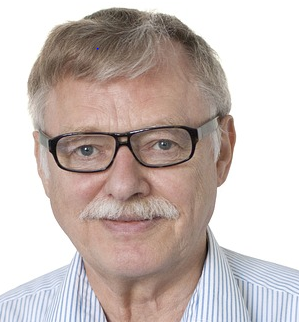
\includegraphics[width=1.6in,height=1.36in]{./media/image2.png}
	\end{Center}
} & 
\multicolumn{1}{|p{4.09in}|}{{\fontsize{10pt}{12.0pt}\selectfont \textbf{Personal Information}} \par \begin{itemize}
	\item {\fontsize{10pt}{12.0pt}\selectfont Name : Manjit} \par 	\item {\fontsize{10pt}{12.0pt}\selectfont Job Title : Assistant Professor of Mathematics} \par 	\item {\fontsize{10pt}{12.0pt}\selectfont Age : 55} \par 	\item {\fontsize{10pt}{12.0pt}\selectfont University : Punjabi University Patiala} \par 	\item {\fontsize{10pt}{12.0pt}\selectfont Email :mjt@gmail.com} \par 	\item {\fontsize{10pt}{12.0pt}\selectfont Location : Punjab, India} \par 	\item {\fontsize{10pt}{12.0pt}\selectfont Highest Level of Education: PhD in Mathematics, Thapar Institute of Engineering and Technology, India.} \par 
\end{itemize}} \\
\hhline{--}
%row no:2
\multicolumn{2}{|p{6.29in}|}{{\fontsize{10pt}{12.0pt}\selectfont \textbf{Skills}} \par \begin{itemize}
	\item {\fontsize{10pt}{12.0pt}\selectfont \textbf{Mathematician – }Phd in Lie Group Analysis Partial Differential Equations, Painleve Analysis, Conservation Laws}
\end{itemize} \par } \\
\hhline{--}
%row no:3
\multicolumn{2}{|p{6.29in}|}{{\fontsize{10pt}{12.0pt}\selectfont \textbf{Experience}} \par \begin{itemize}
	\item {\fontsize{10pt}{12.0pt}\selectfont Assistance Professor of Mathematics at Punjabi University Patiala, Punjab,India}
\end{itemize} \par } \\
\hhline{--}
%row no:4
\multicolumn{2}{|p{6.29in}|}{{\fontsize{10pt}{12.0pt}\selectfont \textbf{User requirements}} \par {\fontsize{10pt}{12.0pt}\selectfont None mentioned in regards to the project - Eternity: Numbers.} \par {\fontsize{10pt}{12.0pt}\selectfont He thinks that using the scientific calculator for computing natural logarithm is easy.} \par {\fontsize{10pt}{12.0pt}\selectfont However mentioned about the relevance of natural logarithm of 2 in calculating compound interest.} \par } \\
\hhline{--}
%row no:5
\multicolumn{2}{|p{6.29in}|}{{\fontsize{10pt}{12.0pt}\selectfont \textbf{Goals}} \par {\fontsize{10pt}{12.0pt}\selectfont Computing compound interest annually and continuously using natural logarithm of (2) quickly, using the Rule72.} \par } \\
\hhline{--}

\end{tabular}
 \end{table}


%%%%%%%%%%%%%%%%%%%% Table No: 2 ends here %%%%%%%%%%%%%%%%%%%%


\vspace{\baselineskip}

\vspace{\baselineskip}

\vspace{\baselineskip}

\vspace{\baselineskip}

\vspace{\baselineskip}

\vspace{\baselineskip}

\vspace{\baselineskip}

\vspace{\baselineskip}

\vspace{\baselineskip}

\vspace{\baselineskip}

\vspace{\baselineskip}

\vspace{\baselineskip}


%%%%%%%%%%%%%%%%%%%% Table No: 3 starts here %%%%%%%%%%%%%%%%%%%%


\begin{table}[H]
 			\centering
\begin{tabular}{p{1.82in}p{3.87in}}
\hline
%row no:1
\multicolumn{1}{|p{1.82in}}{{\fontsize{10pt}{12.0pt}\selectfont \textbf{Photo}} \par {\fontsize{10pt}{12.0pt}\selectfont \textbf{\ \ \ \ \   }} \par 
	\begin{Center}
		
\includegraphics[width=1.82in,height=1.6in]{./media/image3.png}
	\end{Center}
} & 
\multicolumn{1}{|p{3.87in}|}{{\fontsize{10pt}{12.0pt}\selectfont \textbf{Personal Information}} \par \begin{itemize}
	\item {\fontsize{10pt}{12.0pt}\selectfont Name : Nileesha Fernando} \par 	\item {\fontsize{10pt}{12.0pt}\selectfont Job Title : Student } \par 	\item {\fontsize{10pt}{12.0pt}\selectfont Age :25} \par 	\item {\fontsize{10pt}{12.0pt}\selectfont University: Concordia University} \par 	\item {\fontsize{10pt}{12.0pt}\selectfont Email: nfernado@gmail.com} \par 	\item {\fontsize{10pt}{12.0pt}\selectfont Location: Montreal, QC, Canada} \par 	\item {\fontsize{10pt}{12.0pt}\selectfont Highest Level of Education: Pursuing Master of Software Engineering}
\end{itemize} \par } \\
\hhline{--}
%row no:2
\multicolumn{2}{|p{6.29in}|}{{\fontsize{10pt}{12.0pt}\selectfont \textbf{Skills}} \par {\fontsize{10pt}{12.0pt}\selectfont \textbf{\ \ \  }} \par {\fontsize{10pt}{12.0pt}\selectfont \ \ \ \  Full Stack PHP intern at Planet Rate, Montreal. Her part-time internship requires her to design efficient algorithm for company’s new feature using technologies such as} \par \begin{itemize}
	\item {\fontsize{10pt}{12.0pt}\selectfont PHP} \par 	\item {\fontsize{10pt}{12.0pt}\selectfont HTML} \par 	\item {\fontsize{10pt}{12.0pt}\selectfont CSS} \par 	\item {\fontsize{10pt}{12.0pt}\selectfont Node\  JS} \par 	\item {\fontsize{10pt}{12.0pt}\selectfont MySQL}
\end{itemize} \par } \\
\hhline{--}
%row no:3
\multicolumn{2}{|p{6.29in}|}{{\fontsize{10pt}{12.0pt}\selectfont \textbf{Experience}} \par \begin{itemize}
	\item {\fontsize{10pt}{12.0pt}\selectfont Student – Completed course Algorithm Design Technics and Aritificial\ intelligence  } \par 	\item {\fontsize{10pt}{12.0pt}\selectfont Full Stack Php intern (Web Developer)}
\end{itemize}} \\
\hhline{--}
%row no:4
\multicolumn{2}{|p{6.29in}|}{{\fontsize{10pt}{12.0pt}\selectfont \textbf{User requirements}} \par {\fontsize{10pt}{12.0pt}\selectfont None mentioned in regards to the project - Eternity: Numbers. } \par {\fontsize{10pt}{12.0pt}\selectfont She feels that using the scientific calculator to compute natural logarithm of number is easy.} \par } \\
\hhline{--}
%row no:5
\multicolumn{2}{|p{6.29in}|}{{\fontsize{10pt}{12.0pt}\selectfont \textbf{Goals}} \par {\fontsize{10pt}{12.0pt}\selectfont User seems very satisfied with scientific calculator she is using at work for solving complex mathematical equation involving natural logarithm of 2.} \par } \\
\hhline{--}

\end{tabular}
 \end{table}


%%%%%%%%%%%%%%%%%%%% Table No: 3 ends here %%%%%%%%%%%%%%%%%%%%


\vspace{\baselineskip}

\vspace{\baselineskip}

\vspace{\baselineskip}

\vspace{\baselineskip}

\vspace{\baselineskip}

\vspace{\baselineskip}

\vspace{\baselineskip}
\vspace{\baselineskip}\section*{Problem\ 4:  UML Class Diagram}
\addcontentsline{toc}{section}{Problem\ 4:  UML Class Diagram}


%%%%%%%%%%%%%%%%%%%% Figure/Image No: 1 starts here %%%%%%%%%%%%%%%%%%%%

\begin{figure}[H]
	\begin{Center}
		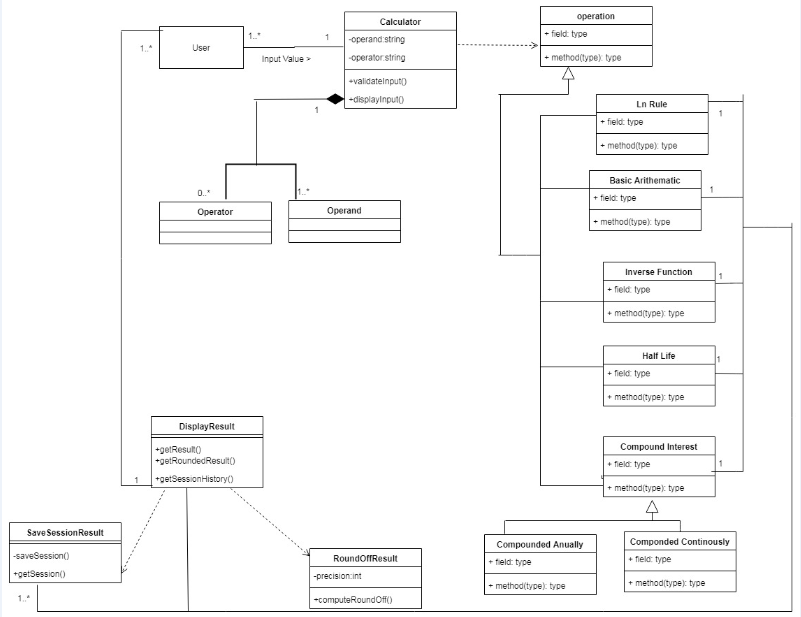
\includegraphics[width=6.43in,height=5.09in]{./media/image4.png}
	\end{Center}
\end{figure}


%%%%%%%%%%%%%%%%%%%% Figure/Image No: 1 Ends here %%%%%%%%%%%%%%%%%%%%

\par


\vspace{\baselineskip}
\vspace{\baselineskip}\section*{Problem 5 : }
\addcontentsline{toc}{section}{Problem 5 : }
\section*{Use Case Diagram}
\addcontentsline{toc}{section}{Use Case Diagram}


%%%%%%%%%%%%%%%%%%%% Figure/Image No: 2 starts here %%%%%%%%%%%%%%%%%%%%

\begin{figure}[H]
	\begin{Center}
		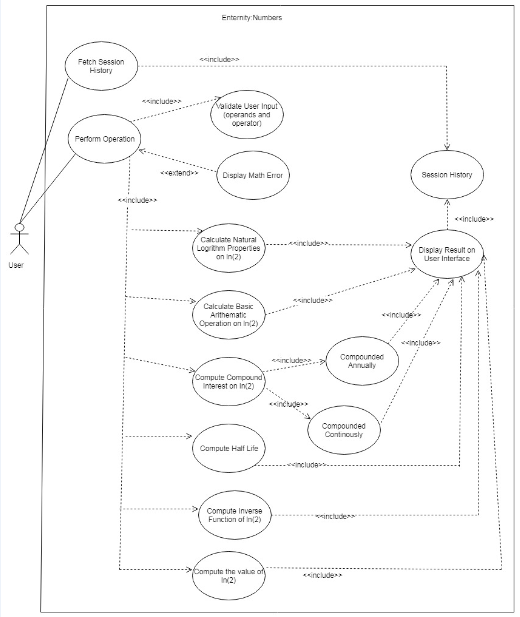
\includegraphics[width=5.51in,height=6.04in]{./media/image5.png}
	\end{Center}
\end{figure}


%%%%%%%%%%%%%%%%%%%% Figure/Image No: 2 Ends here %%%%%%%%%%%%%%%%%%%%

\par


\vspace{\baselineskip}\section*{The operations performed in the use cases -  Calculate natural logarithm of 2, Calculate compound interest using ln(2) - compounded annually and compounded continuously, Compute Half-Life of a Substance, Compute Inverse Function of ln(2), Compute Basic Arithmetic Operation (+,-,$\ast$ ,/) of a number with ln(2).}
\addcontentsline{toc}{section}{The operations performed in the use cases -  Calculate natural logarithm of 2, Calculate compound interest using ln(2) - compounded annually and compounded continuously, Compute Half-Life of a Substance, Compute Inverse Function of ln(2), Compute Basic Arithmetic Operation (+,-,$\ast$ ,/) of a number with ln(2).}

\vspace{\baselineskip}
\vspace{\baselineskip}
\vspace{\baselineskip}
\vspace{\baselineskip}\section*{Activity Diagram }
\addcontentsline{toc}{section}{Activity Diagram }


%%%%%%%%%%%%%%%%%%%% Figure/Image No: 3 starts here %%%%%%%%%%%%%%%%%%%%

\begin{figure}[H]
	\begin{Center}
		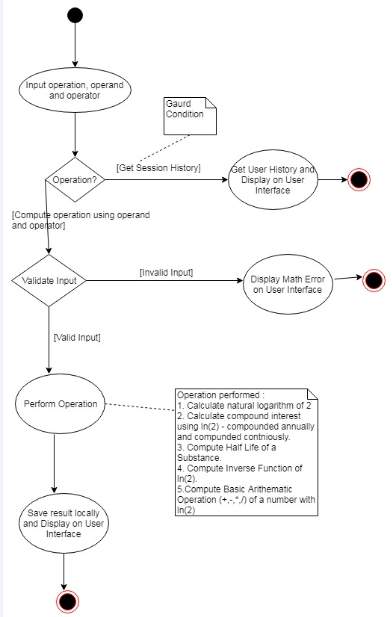
\includegraphics[width=3.6in,height=5.66in]{./media/image6.png}
	\end{Center}
\end{figure}


%%%%%%%%%%%%%%%%%%%% Figure/Image No: 3 Ends here %%%%%%%%%%%%%%%%%%%%

\section*{ }
\addcontentsline{toc}{section}{ }

\vspace{\baselineskip}

\vspace{\baselineskip}

\vspace{\baselineskip}

\vspace{\baselineskip}

\vspace{\baselineskip}

\vspace{\baselineskip}

\vspace{\baselineskip}

\vspace{\baselineskip}

\vspace{\baselineskip}

\vspace{\baselineskip}

\vspace{\baselineskip}

\vspace{\baselineskip}

\vspace{\baselineskip}
\par

\begin{enumerate}
	\item Aigner,\  Martin,\ \ and  Gu¨nter\ \ M.\ \ Ziegler.   Proofs\  from\ \ THE\  BOOK.  Fourth ed.\par

	\item $``$How Do I Prove ln2 Is Irrational?$"$  Quora, \href{http://www.quora.com/How-do-I-prove-}{www.quora.com/How-do-I-prove-} ln2-is-irrational.
\end{enumerate}\par


\printbibliography
\end{document}